\PassOptionsToPackage{usenames,dvipsnames}{xcolor}
\documentclass[tikz,border=2]{standalone}
\usepackage{lmodern} % enhanced version of computer modern
\usepackage[T1]{fontenc} % for hyphenated characters
\usepackage{amssymb}
\usepackage{mathtools} % contains amsmath which comes with align
\usepackage{amsthm}
\usepackage{microtype} % some compression
\usetikzlibrary{shadows,arrows,shapes,positioning,calc,backgrounds,fit,automata,decorations.markings,
decorations.pathreplacing,decorations.pathmorphing}
%%%%%%%%%%%%%%%%%%%%%%%%%%%%%%%%%%%%%%%
% Define the layers to draw the diagram
\pgfdeclarelayer{bg}
\pgfsetlayers{bg,main}
%%%%%%%%%%%%%%%%%%%%%%%%%%%%%%%%%%%%%%%
\begin{document}
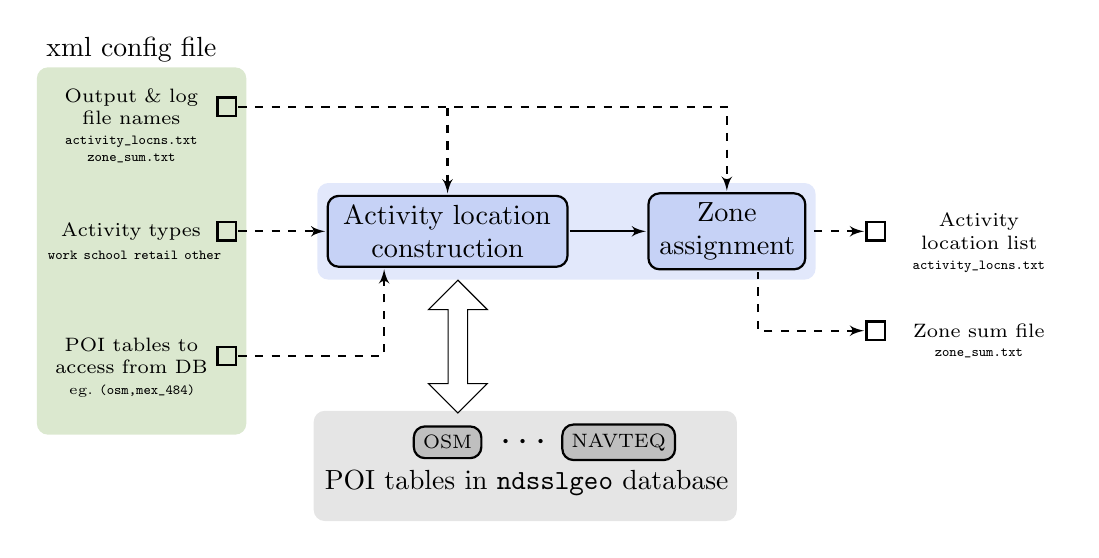
\begin{tikzpicture}
[scale=1,auto, transform shape,
%node distance=.5cm, 
every node/.style={align=center},
modblock/.style={rounded
corners,rectangle,thick,draw=black,fill=RoyalBlue!30,align=center,
text centered},
dbblock/.style={rounded
corners,rectangle,thick,draw=black,fill=black!25,align=center,
text centered,font=\scriptsize},
xmltext/.style={rectangle,text width=6em,font=\scriptsize},
egtext/.style={text width=6em, rectangle,font=\tiny},
ioblock/.style={rectangle,draw=black,thick},
plainblock/.style={rectangle,white,align=center},
dummyblock/.style={rectangle,align=center},
myedge/.style={>=latex', shorten >=.5pt, shorten <=.5pt,thick}
]
\node (xmlOut) [xmltext] {Output \& log file names};
\node (egOut) [egtext,below=-.10 of xmlOut,text width=6em]
{\verb+activity_locns.txt+ \verb+zone_sum.txt+};
\node (bxmlOut) [ioblock,right=-.1 of xmlOut] {};
%
\node (xmlActivity) [xmltext,below= of xmlOut] {Activity types};
\node (bxmlActivity) [ioblock,right=-.1 of xmlActivity]{};
\node (egAct) [egtext,below=-.10 of xmlActivity] {\verb+work school retail other+};
%
\node (xmlPOI) [xmltext,below= of xmlActivity] {POI tables to access from DB};
\node (bxmlPOI) [ioblock,right=-.1 of xmlPOI]{};
\node (egPOI) [egtext,below=-.10 of xmlPOI] {eg.~\verb+(osm,mex_484)+};
%
\node (actloc) [modblock,right=1.3 of xmlActivity, text width=8em]{Activity location construction};
\node (zoneAssign) [modblock,right=1 of actloc, text width=5em]{Zone assignment};
%% \node (nothing) [circle,fill=black!50,above right=of zoneAssign]{};
%
\node (dbOSM) [dbblock,below =2 of actloc] {OSM};
\node (dbOthers) [right =0.1 of dbOSM] {\Large $\cdots$};
\node (dbNAVTEQ) [dbblock,right=of dbOSM] {NAVTEQ};
\node (dbPOI) [below =0 of dbOthers] {POI tables in \verb+ndsslgeo+ database};
%
\node (bactlocOut) [ioblock,right=.75 of zoneAssign] {};
\node (actlocOut) [xmltext,right=0 of bactlocOut] {Activity location list};
\node (egActlocOut) [egtext,below=-.10 of actlocOut] {\verb+activity_locns.txt+};
\node (bzoneOut) [ioblock,below=of bactlocOut] {};
\node (zoneOut) [xmltext,right=0 of bzoneOut] {Zone sum file};
\node (egZoneOut) [egtext,below=-.10 of zoneOut] {\verb+zone_sum.txt+};
%%%%%%%%%%%
\draw[myedge,->,dashed] (bxmlActivity) -- (actloc);
\draw[myedge,->,dashed] (bxmlPOI) -- +(2,0) node (ref3) {} -- (ref3 |- actloc.south);
%%
\draw[myedge,->] (actloc) -- (zoneAssign);
%%
\draw[myedge,->,dashed] (bxmlOut) -- (zoneAssign |- bxmlOut) -- (zoneAssign);
\draw[myedge,->,dashed] (actloc |- bxmlOut) -- (actloc);
\draw[myedge,<-,dashed] (bzoneOut) -- ++(-1.5,0) node (ref2) {}
-- (ref2 |- zoneAssign.south);
\draw[myedge,<-,dashed] (bactlocOut) -- (zoneAssign);
%%
\begin{pgfonlayer}{bg}
\path (xmlOut)+(-1.2,.5) node (ref11)  {};
\path (bxmlPOI)+(+.25,-1) node (ref12) {};
\path [fill=OliveGreen!15,rounded corners] (ref11) rectangle (ref12) node (ref13) {};
%%
\path (zoneAssign.south east) node (ref22) {};
\node [fill=RoyalBlue!15,rounded corners,fit=(actloc)(zoneAssign)] {};%% (actloc.north west)+(-.20,.3)
\node [above =.1 of xmlOut,align=center] {xml config file};
%%
\path (dbOSM)+(-1.7,.4) node (ref21)  {};
\path (dbNAVTEQ)+(1.5,-1) node (ref22) {};
\path [fill=black!10,rounded corners] (ref21) rectangle (ref22) node (ref23) {};
\node[double arrow,draw,below=of actloc,rotate=90,minimum
height=4.8em,xshift=0cm]{};
%%
\end{pgfonlayer}
\end{tikzpicture}
{}
\end{document}

